% @author Benjamin Schröder
%
% Konzepte:
% - Splicing
% - Reduzierbarkeit (reducible graphs)
% - Irreducible Graphs (alle Graphen sind entweder reduzierbar oder unvollständig)

\chapter{Konzept}
\label{chap:konzept}
Das Verfahren von Bokeloh et al. \cite{3_bokeloh_et_al} ist zwar vielseitig einsetzbar und kann auf eine Vielzahl von verschiedenartigen
Modellen angewandt werden, jedoch unterscheiden sich die erzeugten Strukturen in vielen Fällen kaum vom Input. Meist werden lediglich
vorhandene Teilbereiche des Modells neu angeordnet. Die zugrundeliegenden Muster, die ein bestimmtes Modell ausmachen, werden jedoch
nicht erkannt \cite{1_merrell}. Genau hier setzt das nachfolgende Kapitel an und stellt ein Verfahren vor, welches versucht solche grundlegenden Muster
zu erkennen. Zunächst wird ein grober Überblick zum gesamten Ablauf gegeben. Anschließend werden einige grundlegende Konzepte, die für
das weitere Verständnis wichtig sind, vorgestellt, bevor dann letztendlich alle einzelnen Teilschritte im Detail erläutert werden.
Die vorgestellten Konzepte beruhen dabei auf den Erkenntnissen von Paul Merrell in seiner Arbeit aus dem Jahr 2023 \cite{1_merrell}.
Alle Paragraphen in diesem Kapitel, die nicht explizit mit einer Referenz versehen sind, beziehen sich auf genau diese Quelle.

\section{Überblick}

\begin{figure}[t]
    \centering
    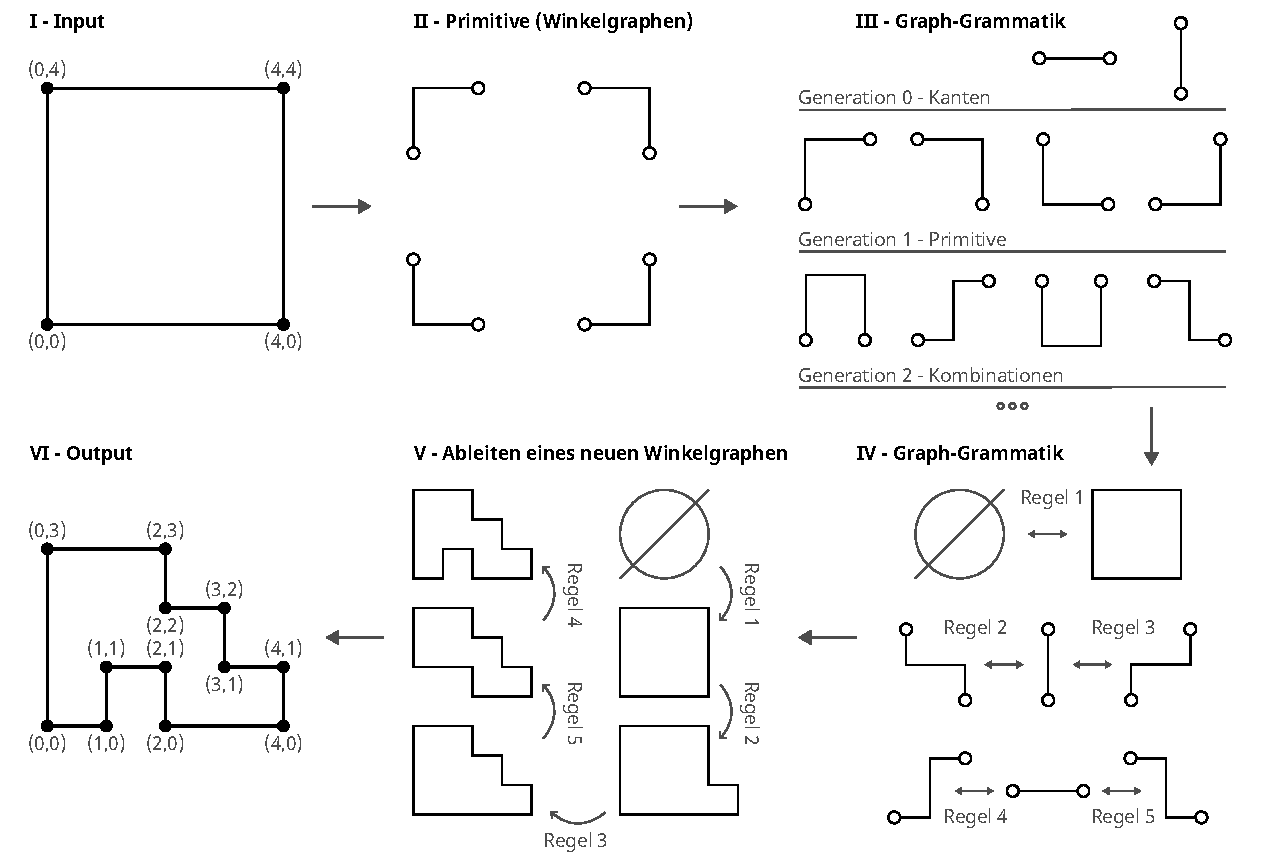
\includegraphics[width=\imgWidth]{images/overview.pdf}
    \caption{Überblick zum Ablauf des Verfahrens.}
    \label{fig:overview}
\end{figure}

Bevor es um die Einzelheiten und spezifischen Konzepte geht, wird zunächst ein grober Überblick zum Ablauf des umgesetzten
Verfahrens geliefert. Das Ganze beginnt mit einer polygonalen Inputstruktur, d.h. einem Gebilde bestehend aus einem oder mehreren Polygonen
(siehe Abbildung \ref{fig:overview}-I).
Diese Inputstruktur wird anschließend umgewandelt in einen Graphen, in welchem die konkrete Geometrie des Inputs keine Rolle
mehr spielt und sich auf die für das Verfahren wichtigen Eigenschaften des Inputs konzentriert werden kann.

Im nächsten Schritt wird der erstellte Graph nun in seine kleinstmöglichen Einzelteile zerlegt. Dazu werden alle Kanten in zwei Halbkanten
aufgeteilt. Das Ergebnis sind viele Teilgraphen, welche jeweils nur noch aus einem Knoten und einigen Halbkanten bestehen.
Einen solchen Teilgraphen nennen wir \textit{Primitiv}. Diese Primitive werden dann Schritt für Schritt in allen möglichen Kombinationen
zusammengeklebt, was zum Entstehen einer Hierarchie an immer komplexer werdenden Graphen führt (siehe Abbildungen \ref{fig:overview}-II und
\ref{fig:overview}-III). \cite{1_merrell}

Beim Aufbau der Hierarchie werden die neu entstehenden Graphen auf bestimmte
Eigenschaften überprüft, die es uns erlauben, daraus Regeln für eine Graphgrammatik abzuleiten (siehe Abbildung \ref{fig:overview}-IV).
Das einfachste Beispiel hierfür sind
vollständige Graphen, also Graphen, die nur noch aus in sich geschlossenen Kreisen bestehen und keine Halbkanten mehr besitzen. Aus diesen lässt
sich eine sogennante Startregel ableiten, welche den leeren Graphen mit dem gefundenen vollständigen Graphen ersetzt. Das Finden von weiteren
Regeln ist deutlich komplizierter und wird später im Detail erläutert. \cite{1_merrell}

Sobald nun eine Menge von Regeln für die Graphgrammatik gefunden wurde, kann man diese verwenden, um verschiedenste zum Inputgraphen
ähnliche Graphen abzuleiten. Dazu werden die gefundenen nach und nach zufällig angewendet, was man in Abbildung \ref{fig:overview}-V sehen kann.
Für einen solchen Graphen müssen dann nur noch konkrete Knotenpositionen und Kantenlängen bestimmt werden (siehe Abbildung \ref{fig:overview}-VI).
\cite{1_merrell}

\section{Grundlagen}
\subsection{Input}
\label{chap:input}
Der Algorithmus kann mit beliebigen polygonalen Strukturen als Input arbeiten. Dies können einfache Rechtecke oder aber auch komplizierte Gebilde
aus verschiedenen Häusern oder ähnlichem sein. Wichtig ist lediglich, dass der Input als Sammlung von Polygonen beschrieben werden kann.

Ein Polygon ist eine geometrische Figur, die vollständig durch ein Tupel \(P\) von \(n\) verschiedenen Punkten beschrieben werden kann:
\[P = (P_1,P_2,\dots,P_n), P_i \in \mathbb{R}^2, 3 \leq i \leq n\]
Diese Punkte bezeichnen wir als \textit{Eckpunkte} des Polygons. Verbindet man zwei
aufeinanderfolgende Eckpunkte in Form einer Strecke \(\overline{P_i P_{i+1}}\) (für \(i = 1,\dots,n-1\)) bzw. \(\overline{P_n P_1}\) miteinander, so
erhält man eine \textit{Seite} des Polygons. All diese Seiten zusammen spannen das Polygon auf. Eine Beschränkung der Anzahl an Eckpunkten
nach oben gibt es dabei nicht, jedoch werden mindestens drei verschiedene Punkte für unsere Definition des Polygons vorausgesetzt. Mit weniger
als drei Punkten können lediglich Figuren ohne Fläche (Punkte, Linien) erzeugt werden, welche für uns nicht von Nutzen sind.
Ebenso sind Kreise oder andere Strukturen mit Rundungen nicht als Polygon darstellbar und können lediglich durch komplexe Polygone angenähert
werden. Der Input kann somit keine Rundungen enthalten.

Die einzelnen Polygone können außerdem mit Farben versehen werden, um verschiedene Arten von abgegrenzte Bereichen im Input zu markieren.

\subsection{Lokale Ähnlichkeit}
% Alte Formulierung:
% Ziel des Verfahrens ist es, Variationen des Inputs zu erzeugen. Dabei soll der Output eine gewisse Ähnlichkeit zum Input beibehalten. Global
% vorzugehen und die vollständigen Input- und Output-Strukturen miteinander zu vergleichen führt hierbei allerdings zu keinem brauchbaren
% Ergebnis. Der Output muss sich zumindest teilweise vom Input unterscheiden, ansonsten ist das Ergebnis nicht zu gebrauchen. Um Vergleiche
% auf einer kleineren Ebene vornehmen zu können, stellen wir hier das Konzept der \textit{lokalen Ähnlichkeit} vor. Das Verfahren gilt als
% erfolgreich, wenn die letztendlich erzeugten Output-Strukturen eine solche lokale Ähnlichkeit zum Input vorweisen können.

Das Ziel, das durch dieses Verfahren erreicht werden soll, ist es, Variationen des Inputs zu erzeugen. Die erzeugten
Outputstrukturen sollen dabei \textit{lokal ähnlich} zum gegebenen Input sein. \cite{1_merrell} Das Konzept der \textit{lokalen Ähnlichkeit} wird im Folgenden
vorgestellt. Das Verfahren gilt nur als erfolgreich, wenn diese zwischen Input und Output nachgewiesen werden kann.

Zwei Polygonstrukturen sind sich lokal ähnlich, wenn sich jeder Teil der einen Struktur zu einem Teil der anderen Struktur zuordnen lässt. Es
müssen sich also alle verschiedenen Arten von Kanten und alle Polygonfarben irgendwo in beiden Strukturen finden lassen. Ein verwandtes Konzept,
das zum Verständnis beitragen kann, ist das der \textit{r-Ähnlichkeit}, welche im Paper von Bokeloh et al. \cite{3_bokeloh_et_al} vorgestellt wurde.
Zwei Strukturen sind hier
\textit{r}-ähnlich, wenn wir für jeden Punkt innerhalb der einen Struktur einen Kreis mit Radius \textit{r} aufspannen können und sich der Inhalt
dieses Kreises (r-Nachbarschaft des Punktes) genauso in der anderen Struktur wiederfinden lässt. Ein Beispiel hierfür befindet sich in Abbildung
\ref{fig:rsimilarity}.

\begin{figure}[t]
    \centering
    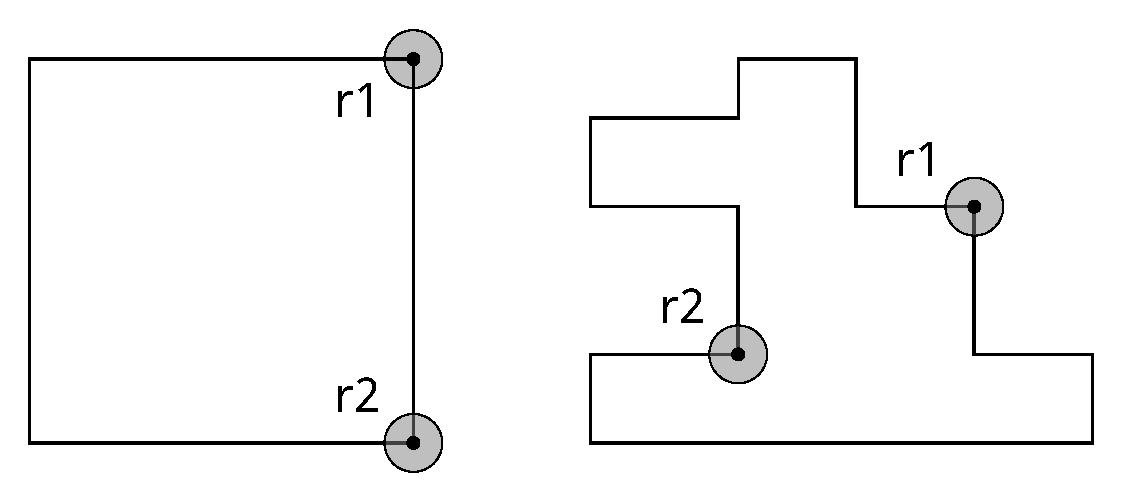
\includegraphics[height=\imgHeight]{images/rsimilarity.pdf}
    \caption{r-Ähnlichkeit.}
    \label{fig:rsimilarity}
\end{figure}

Die von uns verwendete lokale Ähnlichkeit funktioniert nach dem gleichen Konzept, mit der Ausnahme, dass der Radius so klein wie möglich gehalten
wird. Wir schauen uns also lediglich an, welche Kanten und Polygone direkt an einem Punkt anliegen, während uns die restliche Nachbarschaft
egal ist. So können die betrachteten Strukturen beliebig skaliert werden und trotzdem ihre lokale Ähnlichkeit zueinander bewahren, solang alle
Kantenwinkel dabei beibehalten werden. \cite{1_merrell}

\subsection{Der Winkelgraph}
\label{chap:winkelgraph}
Zur Verarbeitung des Inputs wird dieser in einen sogenannten Winkelgraphen umgewandelt, in welchem die spezifischen Positionen der Knoten
keine Rolle spielen. Stattdessen wird nur abgebildet, welche Knoten es überhaupt gibt, welche der Knoten durch Kanten miteinander verbunden
sind, und in welchem Winkel diese Kanten verlaufen.
Die Kanten im Graphen werden mit einem \textit{Kantenlabel} versehen, welches neben den Start- und Endknoten ebenfalls Informationen zum
daraus ableitbaren Tangentenwinkel, sowie zu den Farben der links und rechts anliegenden Polygone enthält. Ein Kantenlabel besitzt die Form
\(\tilde{k} = (l,r,\theta)\), wobei \(\tilde{k}\) die Bezeichnung der Kante, \(l\) und \(r\) die Farben der anliegenden Polygone, und
\(\theta\) der Tangentenwinkel der Kante sind.
Nach der Umwandlung des Inputs in einen Winkelgraphen ist dieser zunächst \textit{vollständig}, d.h. er besteht ausschließlich aus
geschlossenen Kreisen. In späteren Verarbeitungsschritten wird dieser allerdings in unvollständige Teilgraphen zerlegt, welche dann außerdem
\textit{Halbkanten} enthalten können. Im Gegensatz zu den vorher erwähnten Kanten sind diese gerichtet, können aber trotzdem durch ein
gleichartiges Kantenlabel beschrieben werden. In späteren Abschnitten wird noch etwas genauer auf die Relevanz von Halbkanten und deren
spezifische Notation eingegangen. \cite{1_merrell}

\subsubsection{Komplexität von Winkelgraphen}
Später müssen einige der erstellten Winkelgraphen miteinander verglichen werden. Dabei muss bestimmt werden können, welcher
von zwei Graphen komplexer bzw. simpler ist. Dies ist nicht schwierig, sollte jedoch einmal eindeutig definiert werden. Das ausschlaggebendste
Kriterium hierbei ist die Anzahl der Halbkanten der verglichenen Graphen. Ein Graph mit weniger
Halbkanten gilt direkt als simpler als ein Graph mit einer größeren Anzahl an Halbkanten. In vielen Fällen werden die verglichenen Graphen jedoch die gleiche Anzahl
an Halbkanten vorzuweisen haben. Hier wird die Graph-Hierarchie wichtig. Wurde ein Graph früher in die Hierarchie eingefügt, so gilt dieser als
simpler. Dies kann immer eindeutig bestimmt werden und es kommt zu keinen weiteren Konflikten. \cite{1_merrell}

\subsection{Planarität und der Graph Boundary String}
Damit die erzeugten Winkelgraphen später auch ohne Überschneidungen der Kanten dargestellt werden können, muss deren Planarität sichergestellt
werden. Die endgültig erzeugten vollständigen Winkelgraphen bestehen nur noch aus geschlossenen Kreisen. Diese können dann als Polygone
dargestellt werden, vorausgesetzt der jeweilige Kreis war planar. \cite{1_merrell}

Ein geschlossener Kreis ist planar, wenn wir uns beim Traversieren seiner Kanten exakt einmal um 360° gedreht haben. Wenn wir also iterativ
alle Kanten eines solchen Kreises gegen den Uhrzeigersinn betrachten, jeweils die Differenz der Winkel berechnen und diese Differenzen
aufsummieren, so erhalten wir einen Gesamtwinkel von 360°. Es kann allerdings auch vorkommen, dass wir beim Entlanglaufen eines Pfades um
einen geschlossenen Kreis herum einen Gesamtwinkel von mehr als 360° erhalten, so z.B. 720°. Ist dies der Fall, so muss sich der Pfad zwingend
selbst gekreuzt haben. Analog würde es bei der Darstellung der Kanten des entsprechenden Kreises mindestens eine unvermeidliche Überschneidung
geben. Somit wäre der Winkelgraph, der diesen Kreis enthalten hat nicht mehr planar, was in Abbildung \ref{fig:planarity} visuell verdeutlicht wird.
\cite{1_merrell}

\begin{figure}[t]
    \centering
    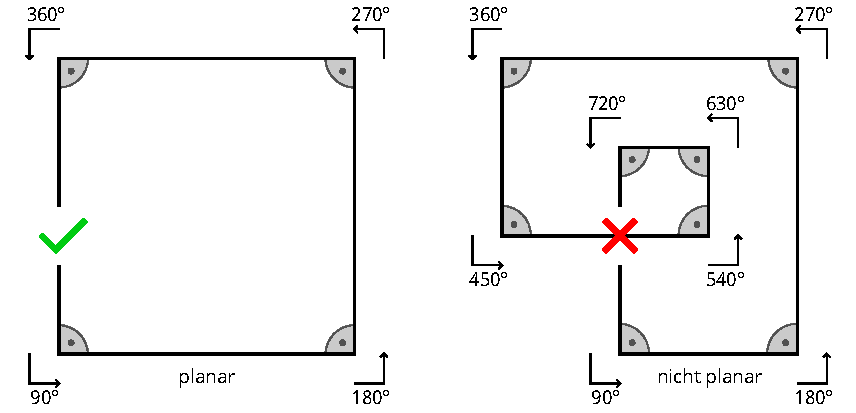
\includegraphics[width=(\imgWidth*3/4)]{images/planarity.pdf}
    \caption{Der Zusammenhang zwischen Drehwinkel und Planarität.}
    \label{fig:planarity}
\end{figure}

Zum Vorbeugen dieses Problems definieren wir hier das Konzept der \textit{Graph Boundary} und die dazugehörige Notation in Form vom
\textit{\gls{ac:gbs}}. Jeder Winkelgraph \(G\) besitzt eine solche Boundary \(\partial G\). Diese beschreibt einen Pfad außen um den entsprechenden
Winkelgraphen herum und enthält alle vorhandenen Halbkanten, sowie Informationen dazu, wie sich die Winkel entlang des Pfades ändern.
Der Pfad verläuft gegen den Uhrzeigersinn und hat keinen festen Startpunkt. Wichtig ist lediglich die relative Anordnung der enthaltenen
Elemente. Um dies abbilden zu können, muss sich der \gls{ac:gbs} nicht als Liste mit festem Start- und Endpunkt vorgestellt werden,
sondern als Kreis mit einer zusätzlichen Verbindung zwischen Anfang und Ende. Angenommen \(abc\wedge\) ist ein \gls{ac:gbs}, dann gilt
\(abc\wedge = bc\wedge a = c\wedge ab = \wedge abc\). \cite{1_merrell}

Um den aktuellen Drehwinkel in Relation zum Startpunkt des Pfades zu ermitteln, können wir uns jeweils die Kantenlabel der traversierten
Kanten anschauen und dort den Tangentenwinkel entnehmen. Dies wird allerdings problematisch, sobald sich der Pfad um mehr als
360° dreht, da die Tangentenwinkel bei 180° bzw. -180° umgebrochen werden. Berechnen wir den aktuellen Drehwinkel entlang der Graph Boundary mithilfe
dieser Tangentenwinkel, so können wir nie eine Differenz von über 360° erhalten. Haben wir uns vom Startpunkt aus z.B. tatsächlich um 400°
gedreht, so würde die hier berechnete Differenz lediglich \(400\degree - 360\degree = 40\degree\) betragen. Wir wissen also nie, ob wir uns
aktuell um den Winkel \(\theta\), \(\theta + 360\degree\), \(\theta + 720\degree\) oder noch mehr gedreht haben.
Dieses Problem lässt sich durch Einführung des Konzepts der \textit{positiven und negativen Drehungen} umgehen. \cite{1_merrell}

\textit{Positive Drehung \(\wedge\).} Dreht sich der Pfad aktuell gegen den Uhrzeigersinn wird der Winkel mit jeder gefundenen Kante größer. Stoßen wir
dabei allerdings auf den Schwellwert von 180°, so bricht der Winkel auf einmal in den negativen Bereich um. Diesen Umbruch bezeichnen wir als
positive Drehung. Folgen wir beim Entlanglaufen des Pfades dem Verlauf einer positiven Kanten und wechseln dann auf eine negativ verlaufende Kante, so
werden wir dabei in einigen Fällen diesen Schwellwert überschreiten. Falls dies geschieht, so fügen wir eine
positive Drehung in Form des Symbols \(\wedge\) in den \gls{ac:gbs} ein. Die Boundary eines planaren Winkelgraphen muss zwingend eine
solche positive Drehung enthalten. \cite{1_merrell}

\textit{Negative Drehung \(\vee\).} Die negative Drehung stellt das Gegenteil zur positiven Drehung dar. Dreht sich der Pfad aktuell im
Uhrzeigersinn, so nähern sich die gefunden Winkel nach und nach dem Schwellwert von -180°. Anschließend bricht der Winkel in den positiven Bereich
um, was wir als negative Drehung bezeichnen und mit dem Symbol \(\vee\) im \gls{ac:gbs} notieren. \cite{1_merrell}

\begin{figure}[t]
    \centering
    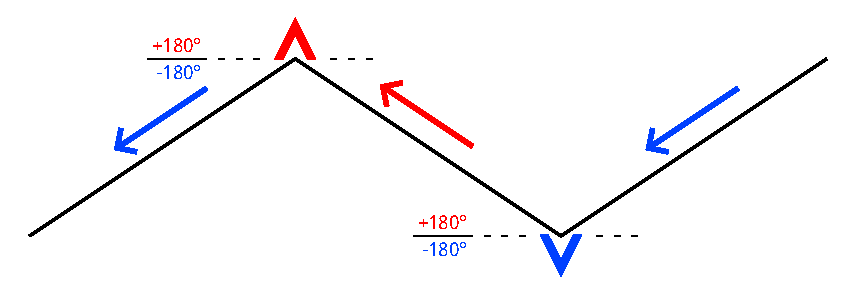
\includegraphics[width=(\imgWidth*3/4)]{images/turns.pdf}
    \caption{Positive und negative Drehungen.}
    \label{fig:turns}
\end{figure}

Die beiden in Abbildung \ref{fig:turns} zu sehenden Drehungen heben sich gegenseitig auf. Befinden sich eine positive und eine negative Drehung
nebeneinander im \gls{ac:gbs}, so können diese entfernt werden. Ebenfalls kann an jeder beliebigen Stelle ein ``\(\wedge\vee\)'' oder ein
``\(\vee\wedge\)'' eingefügt werden, ohne die Bedeutung des jeweiligen \gls{ac:gbs} zu verändern. Eine weitere Eigenschaft, die sich für den \gls{ac:gbs}
für alle planaren Winkelgraphen ergibt ist, dass sich darin immer genau eine positive Drehung mehr befinden muss, als es negative Drehungen gibt.
Dies liegt daran, dass sich der Pfad um einen planaren Graphen insgesamt exakt um 360° dreht und der Drehwinkel somit zumindest einmal irgendwo
den Schwellwert überschreiten muss. Da wir die Graph Boundary entgegen des Uhrzeigersinns ablaufen,
handelt es sich dabei um eine positive Drehung \(\wedge\). \cite{1_merrell}

\subsection{Teil-Operation}
Eine Kante \(\tilde{k}\) kann in zwei Halbkanten \(k\) und \(\overline{k}\) zerteilt werden. Im Gegensatz zu \(\tilde{k}\)
sind diese beiden Halbkanten gerichtet und zeigen in entgegengesetze Richtungen. Dabei zeigt \(k\) stets in positive Richtung und besitzt einen
positiven Tangentenwinkel \(\theta \in [0\degree,180\degree) \), während \(\overline{k}\) immer in negative Richtung zeigt und einen negativen
Tangentenwinkel \(\theta \in [-180\degree,0\degree) \) besitzt. Ein Tangentenwinkel von 0° zählt hier als positiv. Der entgegengesetze Winkel
von 180\degree\ gilt als negativ, da dieser ebenfalls als -180\degree\ interpretiert werden kann. Die Teil-Operation ermöglicht das Zerlegen vom
Input in seine Primitive. \cite{1_merrell}

\subsection{Klebe-Operation}
Zwei entgegengesetze Halbkanten \(k\) und \(\overline{k}\) können wieder zu einer vollständigen und ungerichteten Kante
\(\tilde{k}\) zusammengeklebt werden. Dies ermöglicht das Schließen von Kreisen innerhalb eines Graphen oder die Kombination von mehreren
kleineren Graphen, vorausgesetzt diese besitzen passende Halbkanten. Hier ist erneut der \gls{ac:gbs} von Relevanz, da aus diesem alle
möglichen Klebe-Operationen abgeleitet werden können, welche die Planarität der entstehenden Graphen bewahren. Grundlegend gibt es zwei
verschiedene Arten von Klebe-Operationen: Loop Gluing und Branch Gluing. \cite{1_merrell}

\textit{Loop Gluing} beschreibt das Zusammenkleben zweier Kanten innerhalb eines einzigen Graphen. Das Anwenden einer solchen Operation
führt zum Schließen eines Kreises innerhalb des Graphen. Ob ein Loop Gluing auf einen Graphen angewandt werden kann, lässt sich durch das
Vorhandensein eines der zwei Teilstrings ``\(a \overline{a}\)'' oder ``\(\overline{a}\vee a\wedge\)'' innerhalb des \gls{ac:gbs} ermitteln. Werden
die gefundenen Kanten dann zusammengeklebt, muss der \gls{ac:gbs} entsprechend angepasst werden. Für das Loop Gluing ist diese Anpassung
besonders einfach und es muss lediglich der gefundene Teilstring entfernt werden. Die entsprechenden String-Ersetzungen besitzen die Form:

\begin{center}
    \(a \overline{a} \longrightarrow \epsilon\) \ \ \ bzw. \ \ \ \(\overline{a}\vee a\wedge \longrightarrow \epsilon\) 
\end{center}

\textit{Branch Gluing} beschreibt das Zusammenkleben zweier Kanten von verschiedenen Graphen. Dies führt zur Vereinigung der beiden betroffenen
Graphen in einen neuen, größeren Graphen. Besitzt Graph \(G\) die Kante \(\overline{a}\) und Graph \(H\) die Kante \(a\), so kann ein Branch Gluing
durchgeführt werden. Hierbei gibt es wieder zwei Optionen:

\begin{center}
    \(\overline{a}G\) an \(a\): \(a \longrightarrow G \vee\) \ \ \ bzw. \ \ \ \(a H\) an \(\overline{a}\): \(\overline{a} \longrightarrow \vee H\)
\end{center}

Die Großbuchstaben G und H stehen hier jeweils für den Rest des \gls{ac:gbs} der beiden Graphen. Der \gls{ac:gbs} des neu enstandenen Graphen
stellt die Kombination der beiden kleineren \gls{ac:gbs} dar, allerdings ohne die zusammengeklebten Halbkanten und mit einer zusätzlichen
negativen Drehung. \cite{1_merrell}

\begin{figure}[t]
    \centering
    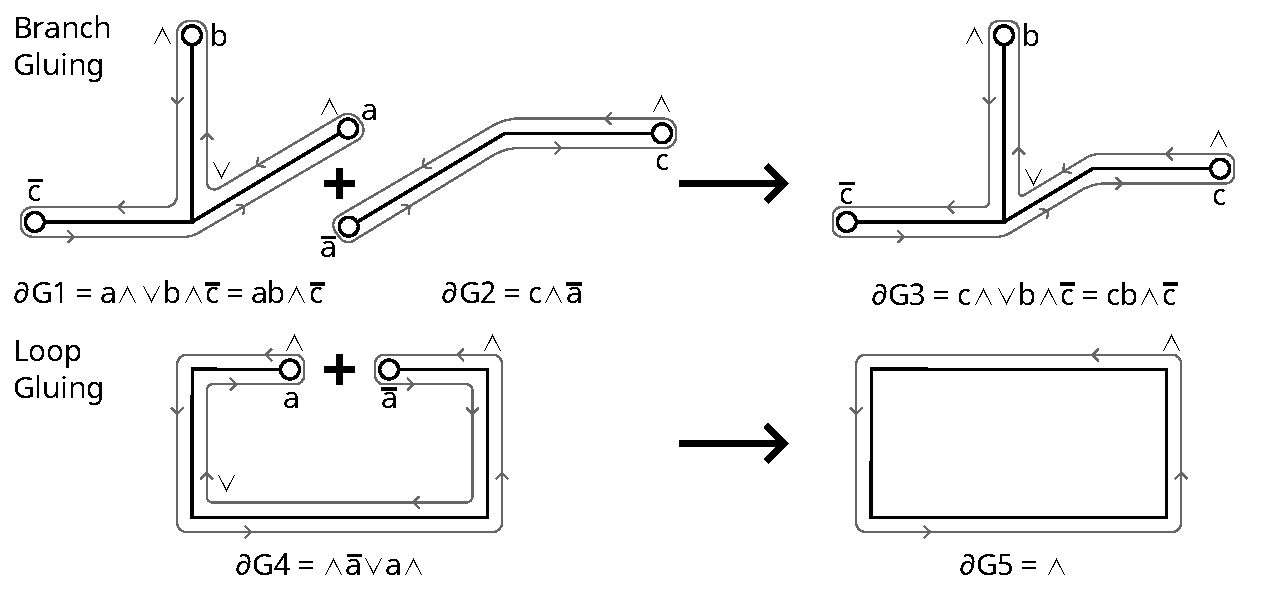
\includegraphics[width=(\imgWidth)]{images/gluing.pdf}
    \caption{Branch und Loop Gluing.}
    \label{fig:gluing}
\end{figure}

\section{Finden der Graphgrammatik}
\subsection{Anpassen des Inputs}
% TODO: Anpassen oder Löschen
Bevor wir mit dem Verfahren beginnen können, muss der Input an bestimmte Anforderungen angepasst werden. Die übergebene Polygonstruktur
kann so nicht direkt verarbeitet werden und muss erst einmal in einen Winkelgraphen umgewandelt werden. Ohne diesen Schritt liegen uns keine
Informationen zu den Kantenwinkeln vor, welche ausschlaggebend für die weiteren Schritte sind. Hierzu werden zunächst einfach alle Knoten und
Kanten aus dem Input übernommen. Anschließend werden die Knotenpositionen genutzt, um den Verlauf der Kanten in Form eines Tangentenwinkels zu
ermitteln. Sobald dies geschehen ist, können die Knotenpositionen dann ignoriert werden, da lediglich die Ausrichtung der Kanten eine Rolle
für die weiteren Schritte spielt. Die restlichen Informationen zur Geometrie werden nicht benötigt und erst beim Erzeugen des finalen Outputs
wieder festgelegt. \cite{1_merrell}

\subsection{Finden der Primitive}
Ist nun der Winkelgraph ermittelt worden, können wir daraus die Primitive ableiten. Diese sind die fundamentalen Grundbausteine für das
gesamte Verfahren. Aus ihnen werden alle weiteren Strukturen abgeleitet, weshalb es besonders wichtig ist, diese korrekt und vollständig zu
ermitteln. Glücklicherweise wird dies durch die vorgestellte Teil-Operation recht trivial. Wenden wir diese auf jede Kante des gegebenen
Winkelgraphen an, so bleiben nur Teilgraphen übrig, welche nur aus einem einzelnen Knoten, sowie einigen Halbkanten bestehen. Diese Teilgraphen
sind dann auch schon die gesuchten Primitive. Hier können allerdings einige identische Teilgraphen entstehen, falls Teile des Input eine ähnliche
Struktur vorzuweisen hatten. Solche Duplikate sind nicht relevant für die weiteren Schritte und werden ignoriert. \cite{1_merrell}

\subsection{Aufbauen der Graph-Hierarchie}
Die vorgestellten Klebe-Operationen ermöglichen es uns, die gefundenen Primitive nach und nach zu komplexeren Graphen zusammenzusetzen.
Diese lassen sich in verschiedene Generationen einer Hierarchie einordnen. In Generation 0 befinden sich alle verschiedenartigen
Kanten, also alle Kanten mit einem einzigartigen Kantenlabel. In Generation 1 befinden sich alle gefundenen Primitive. Anschließend können daraus
die nachfolgenden Generationen automatisch generiert werden. Dazu wird durch alle Winkelgraphen der zuletzt generierten Generation iteriert
und alle durchführbaren Klebe-Operationen auf diese angewandt. Gibt es in einem der iterierten Graphen einen noch offenen Kreis, der aber
durch eine einfach Loop Gluing Operation geschlossen werden kann, so wird diese angwandt. Außerdem werden jeweils alle der gefundenen Primitive
betrachtet und ein Branch Gluing mit diesen ausgeführt, vorausgesetzt deren \gls{ac:gbs} lässt dies zu.
Wird durch eine dieser Operationen ein neuer Graph erzeugt, so gilt dieser als Kind des anderen Graphen. Jeder Graph wird
also neben der Einordnung in eine Generation außerdem in eine Eltern-Kind-Beziehung gebracht. Die Struktur der Hierarchie selbst ähnelt somit
fast der eines Baumes, allerdings kann ein und derselbe Kindsgraph durch verschiedene Elterngraphen erzeugt werden, wodurch wiederum Kreise
innerhalb der Hierarchie entstehen. \cite{1_merrell}

In der Theorie können alle Kombinationen an Primitiven erzeugt werden, wenn wir dieses Vorgehen bis in die Unendlichkeit weiterführen. Somit
würden garantiert alle zum Input lokal ähnlichen Winkelgraphen erzeugt werden und man könnte einfach jeden beliebigen vollständigen Graphen
aus der Hierarchie entnehmen, um jeden validen Output des Verfahrens erzeugen zu können. Praktisch gesehen ist dies natürlich leider nicht
umsetzbar, da uns weder unendlich viele Ressourcen noch Zeit zur Verfügung stehen. Um diesen Ansatz also praktisch zu machen, müssen einige
Anpassungen gemacht werden. \cite{1_merrell}

\subsection{Ableiten der Graphgrammatik}
Statt zuerst eine ``vollständige'' Hierarchie zu erzeugen und aus
dieser dann weitere Schritte abzuleiten, wird die Hierarchie inkrementell erzeugt. Jedes Mal, wenn ein neuer Graph erstellt wird, überprüfen
wir diesen auf bestimmte Eigenschaften, die es uns erlauben daraus Regeln für eine Graphgrammatik abzuleiten. Ein solche Regel ermöglicht es
uns bereits erzeugte Winkelgraphen zu reduzieren, was wiederum bedeutet, dass wir diese nicht mehr benötigen und aus der Hierarchie entfernen
können. Ein detaillierter Einblick zu der Theorie dahinter wird erst in den folgenden Unterkapiteln gegeben, jedoch ist es genau diese Eigenschaft,
die es uns ermöglicht, das Wachstum der Hierarchie einzugrenzen. Optimalerweise erreichen wir irgendwann einen Punkt, an dem alle bereits erzeugten
Graphen durch eine der Regeln reduziert werden konnten. In diesem Fall können wir garantieren, dass sich aus den Regeln alle vollständigen
und zum Inputgraphen lokal ähnlichen Winkelgraphen aus der erzeugten Grammatik ableiten lassen. Meistens werden wir allerdings auf
Szenarien stoßen, in denen die Anzahl der neuen Graphen schneller wächst, als wir andere Graphen entfernen können. Kommt dies vor, so muss das
Erstellen der Hierarchie irgendwann frühzeitig abgebrochen werden und die Graphgrammatik ist eventuell nicht in der Lage, alle lokal ähnlichen
Graphen zu erzeugen. Trotzdem kann die Grammatik dann zum Ableiten einer Vielzahl von lokal ähnlichen Winkelgraphen genutzt werden. \cite{1_merrell}

\subsubsection{Graphgrammatiken}
Bevor wir die Erzeugung dieser Datenstruktur genauer betrachten, soll erst einmal der Begriff der Graphgrammatik klar definiert werden.
Eine Graphgrammatik ist ein formales System, welches spezifisch auf die Erstellung und Manipulation von Graphen in einem mathematisch
präzisen Weg abzielt. Dazu wird eine Menge an Produktionsregeln definiert, welche verschiedene Operationen zum Ersetzen von Teilen
eines Graphen beschreiben. Eine solche Produktion besteht üblicherweise aus drei Bestandteilen: zwei Graphen \(M\) und \(T\) (``Mutter'' und
``Tochter''), sowie einem Einbettungsmechanismus \(E\). Diese Produktion kann nun auf jeden Graphen \(G\) angewandt werden, welcher \(M\)
als Teilgraphen enthält. Um die Produktion anzuwenden, wird \(M\) aus \(G\) entfernt und mit \(T\) ersetzt. Dabei wird \(E\) genutzt, um zu
definieren, wie genau \(T\) in \(G\) eingebettet werden kann. \cite{31_engelfriet_rozenberg}

Das Konzept der Graphgrammatiken existiert bereits seit den frühen 70er Jahren und wurde mit dem Paper von Ehrig et al. \cite{7_ehrig_et_al}
zum ersten Mal formal definiert. Seitdem haben sich sehr viele verschiedene Herangehensweisen in diesem Kontext etabliert, was zu viel Verwirrung
führen kann. \cite{30_könig_et_al} Wir beschränken uns hier auf den ursprünglich präsentierten algebraischen bzw. Gluing-Ansatz von Ehrig 
et al. \cite{7_ehrig_et_al}. Innerhalb dieses Ansatzes haben sich zwei verschiedene Vorgehensweisen etabliert: der Single Pushout Ansatz und der
\gls{ac:dpo} Ansatz, wovon wir den letzteren verwenden. Der Begriff ``Pushout'' stammt aus der Kategorientheorie, welche ebenfalls zum Beschreiben
von Graphgrammatiken genutzt werden kann. \cite{1_merrell}

\begin{figure}[t]
    \centering
    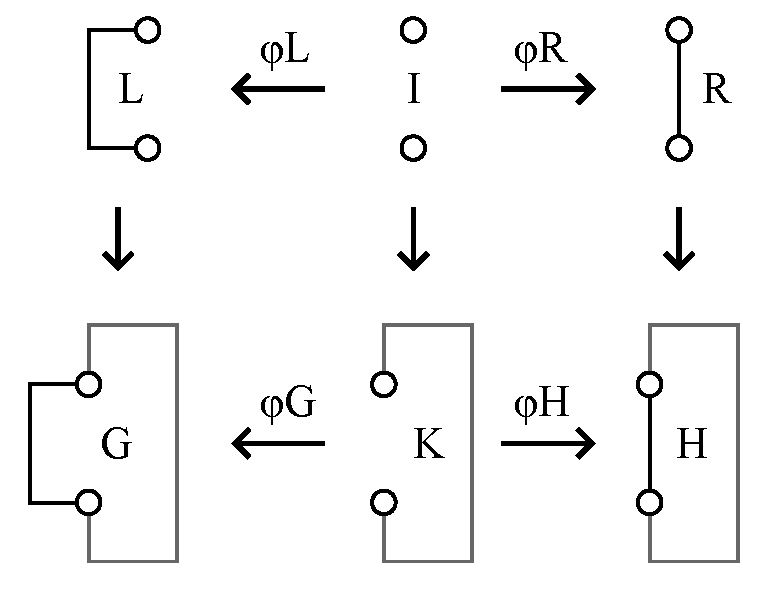
\includegraphics[width=\imgWidth/2]{images/dpo_rule.pdf}
    \caption{Double Pushout Produktionsregel.}
    \label{fig:dpo_rule}
\end{figure}

Die Produktionen im verwendeten \gls{ac:dpo} Ansatz bestehen aus drei Teilen. Einem linken und rechten Graphen (\(L\) und \(R\)), welche jeweils
den Mutter- und Tochtergraphen darstellen, sowie einem Interface-Graphen \(I\), welcher den Einbettungsmechanismus darstellt. Wie in Abbildung
\ref{fig:dpo_rule} zu sehen ist, können diese Graphen mithilfe der Homomorphismen \(\upvarphi L\) und \(\upvarphi R\) untereinander abbilden. \cite{1_merrell}

Ein Homomorphismus von Graph \(A\) (mit der Knotenmenge \(V(A)\) und der Kantenmenge \(E(A)\)) zu Graph \(B\) (mit \(V(B)\) und \(E(B)\)) ist eine
Abbildung \(h: A \rightarrow B\), welche alle Knoten in \(V(A)\) auf eine (meist echte) Teilmenge von \(V(B)\) abbildet: \(x, y \in V(A)
\rightarrow h(x), h(y) \in V(B)\). Sind \(x\) und \(y\) in \(A\) adjazent, so müssen \(h(x)\) und \(h(y)\) in \(B\) ebenfalls adjazent sein:
\((x, y) \in E(A) \rightarrow (h(x), h(y)) \in E(B)\). \cite{35_sabidussi}

Ist \(L\) als Teilgraph in einem anderen Graphen \(G\) enthalten, d.h. gibt es einen Homomorphismus \(\upvarphi m: L \rightarrow G\), so kann die entsprechende
Produktion zum Transformieren von \(G\) verwendet werden. Dazu muss \(L\) zunächst aus \(G\) herausgeschnitten werden. Hierfür wird das Interface
benötigt. Dieses beschreibt die Gemeinsamkeiten zwischen der linken und der rechten Seite der Produktion und ermöglicht das problemlose Austauschen
der beiden Seiten miteinander. Wird \(L\) aus \(G\) entfernt, so erhalten wir den sogenannten Klebegraphen \(K\). In diesen können wir nun \(R\)
hineinkleben, um den transformierten Graphen \(H\) zu erhalten. Das Anwenden einer solchen Produktionsregel ist aber auch in die andere Richtung
möglich. Alternativ kann auch zuerst \(R\) aus \(H\) ausgeschnitten und dann dort \(L\) eingeklebt werden, um \(G\) zu produzieren, vorausgesetzt
es gibt einen Homomorphismus \(\upvarphi n: R \rightarrow H\). \cite{7_ehrig_et_al}

\subsubsection{Theorie hinter der Funktionsweise}
Die später aus der Hierarchie abzuleitenden Produktionsregeln werden so angeordnet, dass sich auf der linken Seite ein komplexerer Graph befindet,
als auf der rechten Seiten. Wird die Regel von links nach rechts angwendet, so vereinfacht sie \(G\). Dies bezeichnen wir als \textit{destruktiv}.
Wird sie von rechts nach links angewendet, so macht sie \(H\) komplexer, was wir wiederum als \textit{konstruktiv} berzeichnen. \cite{1_merrell}

Wie bereits erwähnt, versuchen wir nach dem Erstellen der einzelnen Graphen Regeln zu finden, die bereits erzeugte Graphen in der Hierarchie
vereinfachen können und entfernen diese dann ggf. aus der Hierarchie. Hier werden die Regeln stets nur destruktiv genutzt, was zunächst unlogisch
erscheint. An diesem Punkt können wir uns die Invertierbarkeit der Produktionen zunutze machen. Wenn wir genug Regeln finden können, um alle Graphen
in der Hierarchie zum leeren Graphen reduzieren zu können, indem wir diese destruktiv verwenden, so können wir im Umkehrschluss genau die gleichen
Regeln konstruktiv benutzen, um aus dem leeren Graphen alle anderen Graphen abzuleiten. \cite{1_merrell}

\subsubsection{Ableiten einer Produktionsregel}
Kommen wir nun dazu, wie es möglich ist, solche Regeln automatisch ableiten zu können. Dazu schauen wir uns erneut kurz an, wie eine Produktionsregel
angewandt wird. Wie oben beschrieben, involviert dies zwei Teilschritte. Zunächst wird die eine Seite der Regel aus einem größeren Graphen \(G\)
ausgeschnitten, wodurch dieser zum Klebegraphen \(K\) wird, in welchem nun einige offene Halbkanten enthalten sind. Um \(K\) wieder in einen vollständigen
Graphen \(H\) umwandeln zu können,
müssen all diese Halbkanten anschließend durch Anwenden von entsprechenden Klebeoperationen vervollständig werden. Angenommen, wir haben für den
vorherigen Schritt den Graphen auf der linken Seite der Regel, also \(L\), aus \(G\) ausgeschnitten. Damit der rechte Graph \(R\) die entstandene
Lücke in \(K\) schließen kann, muss dieser exakt die gleichen Halbkanten enthalten, wie \(L\). Besitzt \(R\) weniger Halbkanten, so können einige
der enstandenen Halbkanten in \(K\) nicht vervollständigt werden. Besitzt \(R\) mehr Halbkanten, so würde das Durchführen des Branch Gluings zwischen
\(K\) und \(R\) weitere offene Halbkanten in \(K\) einfügen. Stimmt die Anzahl der Halbkanten in \(L\) und \(R\) überein, aber die Kantenlabel
unterscheiden sich, so kann \(K\) ebenfalls nicht vervollständigt werden. Nur bei hundertprozentiger Übereinstimmung der Halbkanten auf beiden Seiten
der Regel kann diese also problemlos angewandt werden. \cite{1_merrell}

Um aus der Hierarchie eine Regel ableiten zu können, müssen wir also jeweils zwei Graphen mit übereinstimmenden Halbkanten finden. Hier können wir uns
den \gls{ac:gbs} zunutze machen, da dieser alle Halbkantenlabel eines Graphen enthält. Besitzen zwei Graphen einen identischen \gls{ac:gbs}, so besitzen
sie zwingend auch die gleichen Halbkanten. Zusätzlich wird durch Abgleichen der Boundary sichergestellt, dass sich an der Planarität des enstehenden
Graphen nach Anwendung einer Produktionsregel nichts ändert. Zwischen den Kanten befinden sich dann nach wie vor die gleichen Drehungen. \cite{1_merrell}

Statt einen Graphen \(L\) immer nur mit genau einem anderen Graphen \(R\) zu ersetzen, können wir alternativ auch auf mehrere Graphen \(\{R_1, R_2, \dots\}\)
auf der rechten Seite abbilden, vorausgesetzt diese befinden sich in der Hierarchie. Lassen sich die \gls{ac:gbs} \(\{\partial R_1, \partial R_2, \dots\}\)
zu \(\partial L\) zusammensetzen, so sind ebenfalls alle Bedingungen erfüllt, um die Regel problemlos anwenden zu können. Durch dieses Vorgehen lassen sich
sehr viele weitere Regeln ableiten und das Wachstum der Graph-Hierarchie wird zusätzlich eingeschränkt. \cite{1_merrell}

\begin{figure}[t]
    \centering
    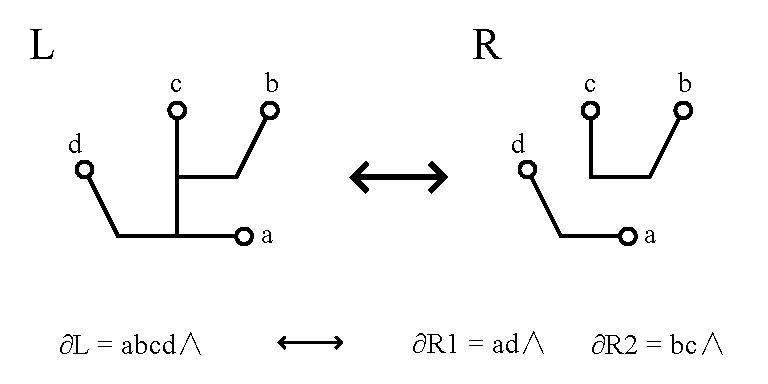
\includegraphics[width=(\imgWidth*3/4)]{images/set_of_graphs.pdf}
    \caption{Ersetzen eines Graphen \(L\) mit mehreren Graphen \(\{R_1,R_2\}\).}
    \label{fig:set_of_graphs}
\end{figure}

Ein Beispiel für eine solche Produktionsregel ist in Abbildung \ref{fig:set_of_graphs} vereinfacht dargestellt. \(\partial L = abcd\wedge\) lässt sich aus
einer Kombination von \(\partial R_1 = ad\wedge\) und \(\partial R_2 = bc\wedge\) bilden. Das Kombinieren von zwei Boundary Strings ist jedoch etwas komplizierter
als das Durchführen einer simplen Konkatenation. Würden wir \(\partial R_1\) und \(\partial R_2\) ohne weitere Anpassungen konkatenieren, so würden wir
einen Boundary String mit zwei positiven Drehungen \(\wedge\) und nicht einer einzigen negativen Drehung \(\vee\) erhalten (z.B. \(a d \wedge b c \vee\)).
Dies würde den Bedingungen für die Planarität widersprechen, da die Differenz zwischen den positiven und negativen Drehungen nun 2 und nicht 1 betragen würde.
Um dieses Problem zu umgehen, wird bei der Kombination zweier \gls{ac:gbs} eine weitere negative Drehung zwischen diesen eingefügt. Nehmen wir an \(A\)
und \(B\) sind Boundary Strings. Die daraus resultierende Kombination hätte dann die Form \(A \vee B\). Dies ist keine willkürliche Anpassung, die
unsere vorher aufgestellten Regeln für einen \gls{ac:gbs} umgeht, sondern eine logische Konsequenz aus diesen. In Abbildung \ref{fig:splicing} ist dies noch einmal
zusätzlich verdeutlicht. \cite{1_merrell}

Widmen wir uns nun wieder dem Beispiel in Abbildung \ref{fig:set_of_graphs}. Aufgrund der kreisförmigen Natur eines \gls{ac:gbs} können wir
\(\partial R_1 = ad\wedge\) auch als \(d\wedge a\) und \(\partial R_2 = bc\wedge\) als \(\wedge bc\) darstellen. Werden diese mit einer zusätzlichen
negativen Drehung in der Mitte kombiniert, so erhalten wir \(\partial R_1 \vee \partial R_2 = d\wedge a\vee \wedge bc = d\wedge abc = abcd\wedge = \partial L\).

Mithilfe dieses Wissens können wir nun systematisch eine Vielzahl von Regeln ableiten:
Nach der Erzeugung eines jeden neuen Graphen \(L\) in der Hierarchie betrachten wir stets alle vorher erzeugten Graphen \(R\) und vergleichen die Boundaries
miteinander. Wird dabei eine hunderprozentige Übereinstimmung \(\partial L = \partial R\) gefunden, so kann direkt eine neue Regel abgeleitet werden.
Alternativ könnte \(\partial R\) auch nur ein Teil von \(\partial L\) sein, was einige Teil-Strings hinterlassen würde. Für diese Teil-Strings wird dann
rekursiv nach weiteren Übereinstimmungen gesucht, bis sich \(\partial L \) entweder komplett aus den gefunden Teil-Strings zusammensetzen lässt oder
es keine weiteren Graphen mehr gibt, die noch überprüft werden können. In letzterem Fall kann dann keine Produktionsregel abgeleitet werden. \cite{1_merrell}

Betrachten wir erneut das Beispiel in Abbildung \ref{fig:set_of_graphs}. Wir haben einen Graphen \(L\) mit der Boundary \(\partial L = abcd\wedge \) erzeugt.
Beim Iterieren durch die Hierarchie finden wir nun den Graphen \(R_1\) mit \(\partial R_1 = ad\wedge \). \(\partial R_1\) ist als Teil in \(\partial L \)
enthalten, wodurch \(R_1\) also einen Teil von \(L\) ersetzen kann. Übrig bleibt der Teil-String \(bc\). Um diesem einen Graphen zuordnen zu können,
muss zunächst eine positive Drehung \(\wedge \) an diesen angefügt werden. Die zusätzliche Drehung wird dann beim Kombinieren automatisch wieder negiert.
Ein Graph \(R_2\) mit \(\partial R_2 = bc\wedge \) kann anschließend ebenfalls gefunden werden, wodurch alle Teile von \(\partial L\) nun komplett sind. Somit kann
aus den gefundenen eine neue Produktionsregel erstellt und \(L\) aus der Hierarchie entfernt werden, da sich dieser nun nachweislich vereinfachen lässt. \cite{1_merrell}

\begin{figure}[t]
    \centering
    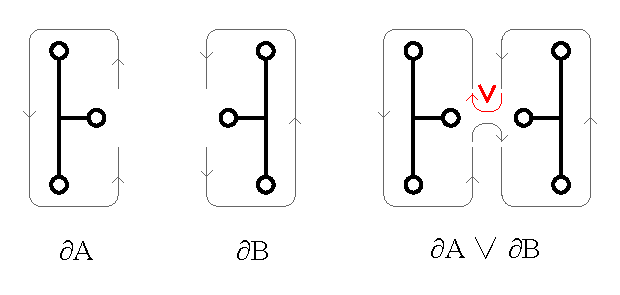
\includegraphics[width=(\imgWidth*3/4)]{images/splicing.pdf}
    \caption{Kombinieren des \gls{ac:gbs} zweier Graphen mit zusätzlicher negativer Drehung.}
    \label{fig:splicing}
\end{figure}

\subsubsection{Starter-Regeln}
Eine Starter-Regel ist eine besondere Produktionsregel, welche den leeren Graphen \(\varnothing\) mit einem vollständigen Graphen ersetzen kann. Davon
kann es theoretisch beliebig viele Regeln geben, jedoch zumindest immer eine. Ohne eine Starter-Regel können keine Graphen aus der Grammatik abgeleitet werden,
da der leere Graph keine Kanten besitzt, auf welche man die Graphen in den anderen Produktionsregeln abbilden könnte. Eine solche Starter-Regel kann durch
das oben beschriebene Vorgehen niemals abgeleitet werden und stellt einen Sonderfall dar. Dieser tritt ein, sobald wir beim Erstellen der Hierarchie
einen vollständigen Graphen \(L\) erzeugen. In diesem Fall wird nicht versucht, \(\partial L\) mit den \gls{ac:gbs} der anderen Graphen in der Hierarchie
abzugleichen. Dies würde ohnehin zu keinem Erfolg führen, da in \(\partial L\) keinerlei Halbkanten enthalten sind. Stattdessen wird \(L\) sofort aus der
Hierarchie entfernt und eine neue Produktionsregel erstellt, welche auf der linken Seite den vollständigen Graphen \(L\) und auf der rechten Seite den
leeren Graphen \(\varnothing\) enthält. \cite{1_merrell}

\section{Erzeugen von Variationen mithilfe der abgeleiteten Regeln}
\subsection{Ableiten eines neuen Winkelgraphen}
Haben wir erfolgreich eine Graphgrammatik abgeleitet, können wir diese nun verwenden, um daraus neue Winkelgraphen zu erzeugen. Dazu wird zunächst eine
Starter-Regel ausgewählt, um eine Grundlage für die weiteren Operationen zu schaffen. Es entsteht ein vollständiger Graph \(G\). Anschließend werden nach
und nach weitere zufällige Produktionsregeln aus der Grammatik ausgewählt und auf den aktuellen Winkelgraphen angewandt. Dabei ist es egal, in welche
Richtung die Regel verwendet wird. Wir können diese sowohl konstruktiv als auch destruktiv benutzen. Um eine Regel anzuwenden, muss der
auszuschneidene Graph \(T\) als Teilgraph in \(G\) enthalten sein. Dies ist der Fall, wenn sich ein Homomorphismus \(m: T \rightarrow G\) finden lässt.
Das Finden eines Homomorphismus zwischen beliebigen Graphen gilt als NP-schweres Problem und
ist somit äußerst kompliziert. \cite{34_cook} Für das Finden von Homomorphismen in planaren Graphen gibt es allerdings effiziente Algorithmen, die in linearer
Zeit zu einem Ergebnis kommen. \cite{8_eppstein} Da wir ausschließlich mit planaren Graphen arbeiten, stellt dies also kein Problem für uns dar. Diesen
Prozess können wir beliebig oft wiederholen und jederzeit abbrechen. Solang zumindest eine Starter-Regel angewandt wurde, erhalten wir in jedem Fall einen
vollständigen Winkelgraphen und somit ein valides Ergebnis für diesen Teilschritt.

\subsection{Festsetzen der Knotenpositionen}
Jetzt gilt es nur noch den eben erzeugten Winkelgraphen in eine Outputstruktur mit festen Knotenpositionen umzuwandeln und gleichzeitig sicherzustellen,
dass diese ohne jegliche Überschneidungen der Kanten dargestellt werden kann. Dazu verwenden wir einen ähnlichen Ansatz wie Bokeloh et al. \cite{4_bokeloh_et_al}
und stellen den Graphen als lineares Gleichungssystem dar, für welches wir anschließend eine Lösung finden. Die einzelnen Gleichungen dieses Systems lassen
sich jeweils aus den Kanten des Winkelgraphen ableiten. Dazu betrachten wir die Positionen des Startknotens \(v_0\) und des Endknotens \(v_1\), sowie den
Tangentenwinkel \(\theta\). Dieser kann wie folgt als zweidimensionaler Richtungsvektor dargestellt werden: \(u = [cos(\theta), sin(\theta)]\). Es handelt
sich hierbei um einen Einheitsvektor, der mit einer Kantenlänge \(s\) multipliziert auf die Position von \(v_0\) addiert werden kann, um \(v_1\) zu erhalten.
Die gesamte Gleichung zum Beschreiben einer Kante lautet dann: \(v_0 + su = v_1\) bzw. \(v_0 + su - v_1 = 0\). \cite{1_merrell} All diese Kantengleichungen können in eine
Matrix-Gleichung der Form \(Ax = 0\) gebracht werden, wobei \(x\) alle Unbekannten (Knotenpositionen und Kantenlängen) und \(A\) alle Koeffizienten dieser
Unbekannten enthält. \(0\) stellt den Nullvektor des entsprechenden Vektorraums dar. Für jede Kantengleichung werden zwei neue Zeilen in die Matrix-Gleichung
eingefügt, da wir mit zweidimensionalen Vektoren arbeiten. Eine Zeile beschreibt die x-Koordinaten, die andere Zeile die y-Koordinaten der Vektoren.
Das Gleichungssystem, das durch dieses Vorgehen entsteht, ist stets
unterbestimmt, d.h. es gibt mehr Unbekannte als Gleichungen im System. Die Konsequenz daraus ist, dass sich keine eindeutige Lösung finden lässt.
Stattdessen können wir nur einen Raum an möglichen Lösungen finden, aus welchem wir dann stichprobenartig einzelne Lösungen auswählen können. Der Raum an
möglichen Lösungen lässt sich durch das Berechnen des Kerns der Matrix \(A\) finden. Der Kern einer Matrix \(M\) ist die Menge aller Vektoren \(x\), für die gilt:
\(Mx = 0\).\footnote{\url{https://www.studysmarter.de/studium/mathematik-studium/lineare-algebra/kern-einer-matrix/} [Letzter Zugriff am 01.07.2024]} Um nun den
Kern von \(A\) zu finden, bringen wir \(A\) zunächst in die reduzierte Zeilenstufenform. Die reduzierte Zeilenstufenform einer Matrix ist stets eindeutig und
erfüllt die folgenden Eigenschaften \cite{47_meyer}:

\begin{itemize}
    \item alle Zeilen, die ledglich aus Nullen bestehen, befinden sich ganz unten
    \item jede Zeile beginnt mit einer Folge von Nullen (ggf. mit Länge 0), gefolgt vom sogenannten \textit{Pivot-Element}
    \item das Pivot-Element einer Zeile befindet sich stets rechts von den Pivot-Elementen aller darüberliegender Zeilen
    \item das Pivot-Element ist stets 1
    \item jede Spalte mit einem Pivot-Element enthält außer dem Pivot-Element nur Nullen
\end{itemize}

Zum Umwandeln einer Matrix in diese Form verwenden wir den Gauß-Jordan-Algorithmus. Dieser ist bereits in vielen anderen Quellen, wie z.B. \cite{47_meyer},
detailliert behandelt worden und soll von uns nicht näher betrachtet werden. Wichtig ist das Ergebnis, welches wir durch dessen Anwendung erhalten. Aus
diesem können wir nun den Kern der Matrix berechnen. Dies wird nachfolgend an einem Beispiel demonstriert:

\[
A =
\begin{bmatrix}
    1 & 2 & -1 & 1 & -4 \\
    2 & 3 & -1 & 1 & -11 \\
    -2 & 0 & -3 & 1 & 22 
\end{bmatrix}
\longrightarrow rref(A) =
\begin{bmatrix}
    1 & 0 & 0 & -2 & -8 \\
    0 & 1 & 0 & 2 & 1 \\
    0 & 0 & 1 & 1 & -2 
\end{bmatrix}
\]

Die reduzierte Zeilenstufenform wird hier abgekürzt durch ``rref'' (reduced row echelon form). Der Kern von \(A\) kann nun berechnet werden, indem die folgende
Gleichung gelöst wird:

\[
\begin{bmatrix}
    1 & 0 & 0 & -2 & -8 \\
    0 & 1 & 0 & 2 & 1 \\
    0 & 0 & 1 & 1 & -2 
\end{bmatrix}
\begin{bmatrix}
    x_1 \\ x_2 \\ x_3 \\ x_4 \\ x_5
\end{bmatrix}
=
\begin{bmatrix}
    0 \\ 0 \\ 0
\end{bmatrix}
\]

Durch die Umwandlung in die reduzierte Zeilenstufenform kann die Lösung aus dieser Darstellung mehr oder weniger abgelesen werden. Jede Spalte ohne ein Pivot-Element
repräsentiert eine freie Variable, was aufgrund der Unterbestimmung des Gleichungssystems zustande kommt. Wählen wir als freie Variablen \(x_4 = t\) und
\(x_5 = s\), so ergibt sich für die weiteren Variablen: \(x_1 = 8s + 2t, \ x_2 = -s - 2t, \ x_3 = 2s - t\). Der Kern von A lautet dann:

\[
Kern(A) =
\begin{bmatrix}
    8s + 2t \\
    -s - 2t \\
    2s - t \\
    t \\
    s
\end{bmatrix}
=
\begin{bmatrix}
    2 \\ -2 \\ -1 \\ 1 \\ 0
\end{bmatrix}
t +
\begin{bmatrix}
    8 \\ -1 \\ 2 \\ 0 \\ 1
\end{bmatrix}
s
\]

Nun können wir beliebige Werte für \(s\) und \(t\) einsetzen, um eine konkrete Lösung für das Gleichungssystem zu erhalten. Leider bedeutet das Finden einer solchen
Lösung nicht unbedingt, dass wir nun auch eine valide Darstellung für die Outputstruktur gefunden haben. Die gefundene Lösung könnte eventuell negative Werte für
die Kantenlängen enthalten, welche nicht dargestellt werden können. Um dies zu umgehen, müssen wir die vorgeschlagenen Lösungen also stets auf ungültige Werte überprüfen
und ggf. eine neue Lösung generieren. Neben dem Überprüfen auf negative Kantenlängen könnten wir hier außerdem weitere durch den Endnutzer angegebene Kriterien überprüfen
und so z.B. alle Kantenlängen auf einen bestimmten Wertebereich beschränken. \cite{1_merrell}
